\documentclass[a4paper,12pt]{article}
\usepackage[utf8]{inputenc}
\usepackage{xcolor}
\usepackage{url}
\usepackage[T2A]{fontenc}
\usepackage{graphicx}
\usepackage[margin=80pt]{geometry}
\usepackage{booktabs}
\usepackage{natbib}

\usepackage[english,serbian]{babel}

\begin{document}

\title{\textbf{Zene u programiranju\\} \small{Seminarski rad u okviru kursa\\Tehnisko i naucno pisanje\\ Matematicki fakultet}}

\author{Jelena Velickovic\\ mi21203@alas.matf.bg.ac.rs \and Bojana Zagorac\\ mi22135@alas.matf.bg.ac.rs \and Milos Bigovic\\ mi22149@alas.matf.bg.ac.rs \and Zorana Jevtic\\ mi22148@alas.matf.bg.ac.rs}

\date{\textit{\center{Novembar, 2022.}}}

\maketitle

\begin{abstract}
    U ovom tekstu je ukratko objasnjen doprinos zena u programiranju uz priloge. Takodje, bice reci o
    brojnosti zena koje se time bave, kao i o Adi Bajron, najistaknutijom zenom programerom. Sustina 
    ovog teksta je razbijanje predrasude da se programiranjem bave iskljucivo muskarci, odnosno da je 
    programiranje "muski posao". 
\end{abstract}


\color{blue}\tableofcontents

\newpage
\color{black}\section{Uvod}

\newpage
\section{Ada Bajron}

\begin{flushleft}
    Ejda Bajron(1815-1852.), poznata kao Ada, smatra se prvim programerom zbog svog programa kojim se pomocu analiticke masine izracunavaju Bernulijevi brojevi. Odnosno, ucestvovala je u realizaciji projekta analiticke masine funansijski i svojim idejama. Njena najznacajnija ideja u realizaciji tog projekta je bio prenos kontrole i rad sa ciklusima. Iako se primarno bavila matematikom, to nije znacilo da se tu zaustavljaju njena interesovanja. Za razliku od mnogih u to doba, bila je inovativna smatrajuci da se analiticka masina moze upotrebljavati za opstije stvari, kao i u naucne svrhe. To je u buducnosti i realizovano, dakle savremeni racunari se upravo uklapaju u tu njenu zamisao.Upoznavsi poznatog matematicara Carlsa Bebidza, nakon nekog vremena mu se pridruzila u projektu kao njegov tumac. To jest, jasno je opisala kako ce masina funkcionisati, cime je doprinela računarskoj nauci. Objasnila je da je sustina rada analiticke masine tkanje algebarskih obrazaca poput Zakardove masine koja je radila po principu kreiranja slika na osnovu busenih kartica. Predmet svojih proucavanja i rada je nazivala naukom i operacijama, medjutim to je zapravo racunarstvo. Nije ni cudno to sto je razmisljala na tako genijalan nacin, s obzirom na to da je spojila mastovitost sa racionalnoscu. Umetnicku crtu je nasledila od oca lorda Bajrona, romanticarskog pesnika, dok je zahvaljujuci majcinom uticaju uspela da stvori ravnotezu i izbegne povrsan pristup. Bez obzira na to sto su neki naucnici pokusavali da ospore njen rad i doprinos, mnogi su odbacivali ovo tumacenje. Razlog osporavanja je bio cuvanje moci u rukama muskarca kao i predrasude prema zenama koje se bave programiranjem zbog spoznaje vaznosti i znacaja te naucne oblasti. Vrhunac njene karijere je programski jezik nazvan Ada u njenu cast, kao i priznanje koje dobija svake godine 15. oktobra, pocevsi od 2009. godine kako bi se istakao naucni rad i doprinos zena koji je zanemaren i nipodastavan. Na slici 1, prikazana je Ada Bajron.
\end{flushleft}

\begin{figure}
    \centering
    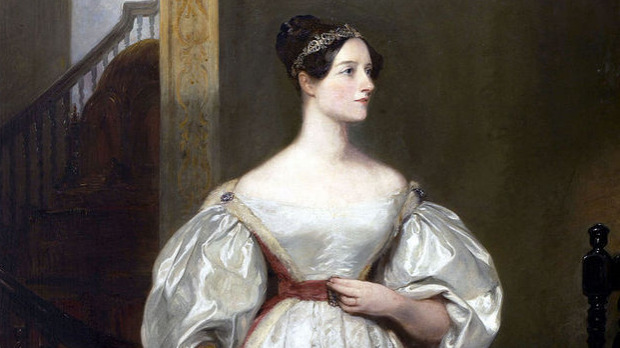
\includegraphics[width = .6\textwidth]{slika/adabajron.jpg}
    \caption{Ада Бајрон}
    \label{fig:my_label}
\end{figure}


\section{ENIAC Programeri}

\subsection{Šta je zapravo ENIAC}
\begin{flushleft}

U periodu između 1943. i 1946. godine od strane američke vojske i tima univerziteta u Pensilvaniji koji su predvodili Džon Mokli i Džej Ekert konstruisan je prvi elektronski računar opšte primene - ENIAC. Osnovna svrha bila mu je jedna specijalna namena - izračunavanje trajektorije projektila. Bilo je moguće da se mašina programira i za druge zadatke ali to je zahtevalo intervencije sa preklopnicicma i kablovima koje su mogle da traju danima. Na programiranju samog računara radilo je šest žena - Ketlin Antoneli, Rut Teitelbaum, Franses Spens, Žan Bartik, Marlin Melcer, Beti Holberton.

\end{flushleft}

\subsection{Ketlin Antoneli}
\begin{flushleft}

Ketlin Antoneli(1921-2006), poreklom iz Irske, je bila Američki programer. Svoje školovanje je započela 1927. godine u Katoličkim školama u Sjedinjenim Državama. Zatim je pohađala Katoličku srednju školu za devojke Džona V. Halahana. 1938. godine se upisala na Čestnat koledž u Filadelfiji, kojeg je i zavrsila 1942. godine.

\end{flushleft}

\subsection{Rut Teitelbaum}
\begin{flushleft}

Rut Teitelbaum(1924-1986), rođena u Njujorku, je bila jedna od prvih programera na svetu. Pohađala je Hanter koledž i zavrsila je sa bachelor degree iz matematike.

\end{flushleft}

\subsection{Franses Spens}
\begin{flushleft}

Franses Spens(1922-2012) je završila srednju školu za devojčice u Južnoj Filadelfiji 1938. godine i upisala Templ Univeritet. Ali ubrzo je dobila stipendiju Čestnat Koledža, gde je upoznala Ketlin Antoneli. Tokom studija se zaposlila kao profesor matematike u srednjoj školi. Ona je htela da bude profesorka matematike, ali 1942. godine odmah nakon zavrsenih studija je zapošljena od strane vojske.

\end{flushleft}

\subsection{Žan Bartik}
\begin{flushleft}

Žan Bartik(1924-2011), usled velikih novčanih problema, je završila Stenberi srednju školu, nakon čega je upisala Učiteljski Koledž na severozapadnom delu Misurija. Upisala je koledž sa namerom da se opredili za novinarstvo, medjutim opredelila se ipak za matematiku. Nakon završetka studija, aplicirala je za posao u IMB kompaniji i na koledžu u Filadelfiji. IBM ju je odbio ali ne i koledž, tako se prvi put susrela sa ENIAC mašinom. 

\end{flushleft}

\subsection{Marlin Melcer}
\begin{flushleft}

Marlin Melcer(1922-2008), poreklom iz filadelfije, je zavrišila Templ Univeritet u Filadelfiji 1942. godine. Zaposlila ju je vojska u Mur školi elektrotehnike na Univerzitetu u Filadelfiji, a ubrzo se učlanila u ekipu koja je radila na mašini ENIAC. 

\end{flushleft}

\subsection{Beti Holberton}
\begin{flushleft}

Beti Holberton(1917-2001) je studirala 40-ih godina proslog veka novinarstvo na Filadelfijskom Univerzitetu, što joj je omogućilo da puno proputuje. Međutim kako je krenuo rat, tako su muškarci išli u rat, a žene su bile zapošljavane za izračunavanje trajektorije samih projektila.

\end{flushleft}


\section{Zbog čega ima manje žena u IT sektoru?}

\subsection{Statistika}

U poslednjih 20 godina, u SAD-u ali i kod nas, je zabeležen nagli pad broja žena koje stiču fakultetske diplome iz računarskih nauka i
informacionih tehnologija. Prema Nacionalnom centru za statistiku obrazovanja, iako žene čine većinu diplomiranih fakulteta, 
one su stekle samo 19posto diploma iz informatike koje su dodeljene 2016.

Medjutim, žene nisu uvek bile toliko nedovoljno zastupljene u IT sektoru. Posle Drugog svetskog rata, 
tokom digitalne revolucije (1950-1970) kompjutersko programiranje je postalo popularnije medju oba pola. 
Do sredine `80-ih godina procenat žena na kompjuterskim naukama rastao je veoma brzo i pretekao čak i medicinu, 
a onda kada su žene počele da u ovoj oblasti čine više od 35posto studenata, procenat je počeo naglo da pada sve do danas. 

\begin{table}[h]
\centering
\begin{tabular}{c|c}
\toprule
Godina    & procenat zena u IT-u \\ 
\midrule
1984      & 37                   \\ 
1990-2010 & 18                   \\ 
2019      & 13                   \\ 
\bottomrule
\end{tabular}
\end{table}



\subsection{Zašto tako malo žena ulazi u ove oblasti? }
Uobičajeno objašnjenje je da su žene manje zainteresovane od muškaraca, 
što nije netačno ali potpuni odgovor na ovo pitanje bi bila kultura, 
koja odvraća mnoge žene i mlade devojke da se zainteresuju za ovaj važan posao.
Iako je teško tačno odrediti zašto postoji tako velikia rodna razlika u računarskoj nauci, 
postoji mnogo razloga za koje je dokazano da doprinose ovom problemu. 
Od štetnih stereotipa do nedostatka podrške za devojčice na školskom nivou i nedostatka ženskih uzora.

Jedan od razloga je začarani krug nedovoljne zastupljenosti sa kojim se žene susreću kada udju u svet tehnologije. 
Što je manje mladih žena koje predstavljaju IT sektor, manja je verovatnoća da će se one prijaviti za posao u toj oblasti. 
Da bi se ovaj problem rešio potrebno je da se žene u IT-u više promovišu, 
odnosno da se poboljša grana marketinga koja se bavi zapošljavanjem žena.


Nagli pad interesovanja žena se desio paralelno kada je upotreba personalnih računara u kućama počela da raste. 
Ti računari su u početku najvećim delom bili korišćeni za igrice, a promovisani su tako da su namenjeni pre svega za dečake. 
Zbog čega su dečaci, od tog perioda imali iskustvo rada sa kompjuterima pre upisa fakulteta, dok devojčice uglavnom nisu, 
pa su se odlučivale za druge oblasti studija. Ideja da su kompjuteri za dečake postala je narativ. 
Razarajuća recesija u industriji video igara koja je trajala od 1983. do 1985. godine, je navela mnoge potencijalne 
kompjuterske programere da preispitaju svoj put u karijeri. 


\subsection{Budućnost žena u IT oblasti}
Jasno je da industrija kompjuterskih nauka raste izuzetnom brzinom. Zbog čega nikada nije bilo važnije da se reši rodna razlika.
Poslovni svet počinje da reaguje na ovu činjenicu. Postojao je spor i stalan tok rada na poboljšanju prepoznavanja i zastupljenosti
žena u IT-u kako iz velikih preduzeća tako i iz manjih organizacija. Neke od najvećih tehnoloških kompanija, uključujući Apple, 
Facebook, Google i Intel, takodje su se obavezale da će poboljšati budućnost žena u IT-u. Twitter, Instagram, TikTok su uveli razne 
heštegove kojim podržavaju i podstiču rad žena u IT kompanijama. Budućnost žena u informatici zavisi od sposobnosti IT industrije 
da inspiriše mlade žene da studiraju računarstvo i informatiku tokom svoje školske karijere, a zatim predju i na fakultete iz ovih oblasti.

\newpage
\bibliographystyle{apalike}
\bibliography{bib}

\cite{ashcraft2016women}
\cite{branson2018future}

\end{document}
